\subsection{ЭФФЕКТЫ КМД В МОДЕЛИ ГЭЦ}

Чтобы обнаружить паттерны КМД в моделируемой ГЭЦ за период 1980--2020, величины вкладов в ИП усреднялись по дням, отвечающим каждой из восьми фаз КМД. Такие фазы определяются на основе полярного угла на плоскости (RMM1, RMM2) (см. рис. \ref{fig:wh04_fig7}); в среднем в течение цикла КМД точка на данной плоскости движется по окружности вокруг начала координат против часовой стрелки, проходя все фазы. Обычно рассматривают не только фазу, но и амплитуду (расстояние от точки до начала координат), что позволяет разделять КМД на слабое и сильное (см. рис. \ref{fig:wh04_fig7}). В данной работе амплитуда индекса RMM не рассматривалась, так как не было обнаружено какой-либо зависимости в обнаруженных эффектах от неё.

Одной из главных черт КМД является перенос с запада на восток крупномасштабной конвективной структуры в тропиках. Исходя из параметризации ИП (\ref{eq:ip}), вклады в ИП от столбцов модели во многом зависят от CAPE и осадков~---~параметров, связанных с глубокой конвекцией. Поэтому разумно предположить, что паттерны КМД будут заметны во вкладах в ИП.

Так как КМД является нерегулярным процессом, то не следует рассматривать отдельные циклы КМД~---~они могут значительно отличаться друг от друга. Альтернативой такому подходу является переход к некоторому универсальному для КМД временному масштабу~---~масштабу 8 фаз, поэтому среднесуточные значения вкладов в ИП усреднялись по дням, приходящимся на каждую из фаз КМД. Затем, вычитается среднее за длительный период времени значение каждого вклада из усредненных по фазам КМД значений. Таким образом осуществляется переход к аномалиям вкладов, которые легко интерпретировать: положительная аномалия означает, что данный столбец модели даёт вклад в ИП больше, чем обычно, а отрицательная аномалия означает, что вклад данного столбца в ИП ниже обычного значения.

Рис. \ref{fig:map_of_contributions} показывает, как такие аномалии во вкладах меняются с фазой КМД. Видно, что положительная и негативная аномалии перемещаются с запада на восток друг за другом с ростом номера фазы КМД. Такой эффект отражает аналогичное перемещение областей усиленной и ослабленной конвективной активности в течение цикла КМД (см. рис. \ref{fig:map_of_olr_anomaly}).

\begin{figure}[tb]
	\centering
	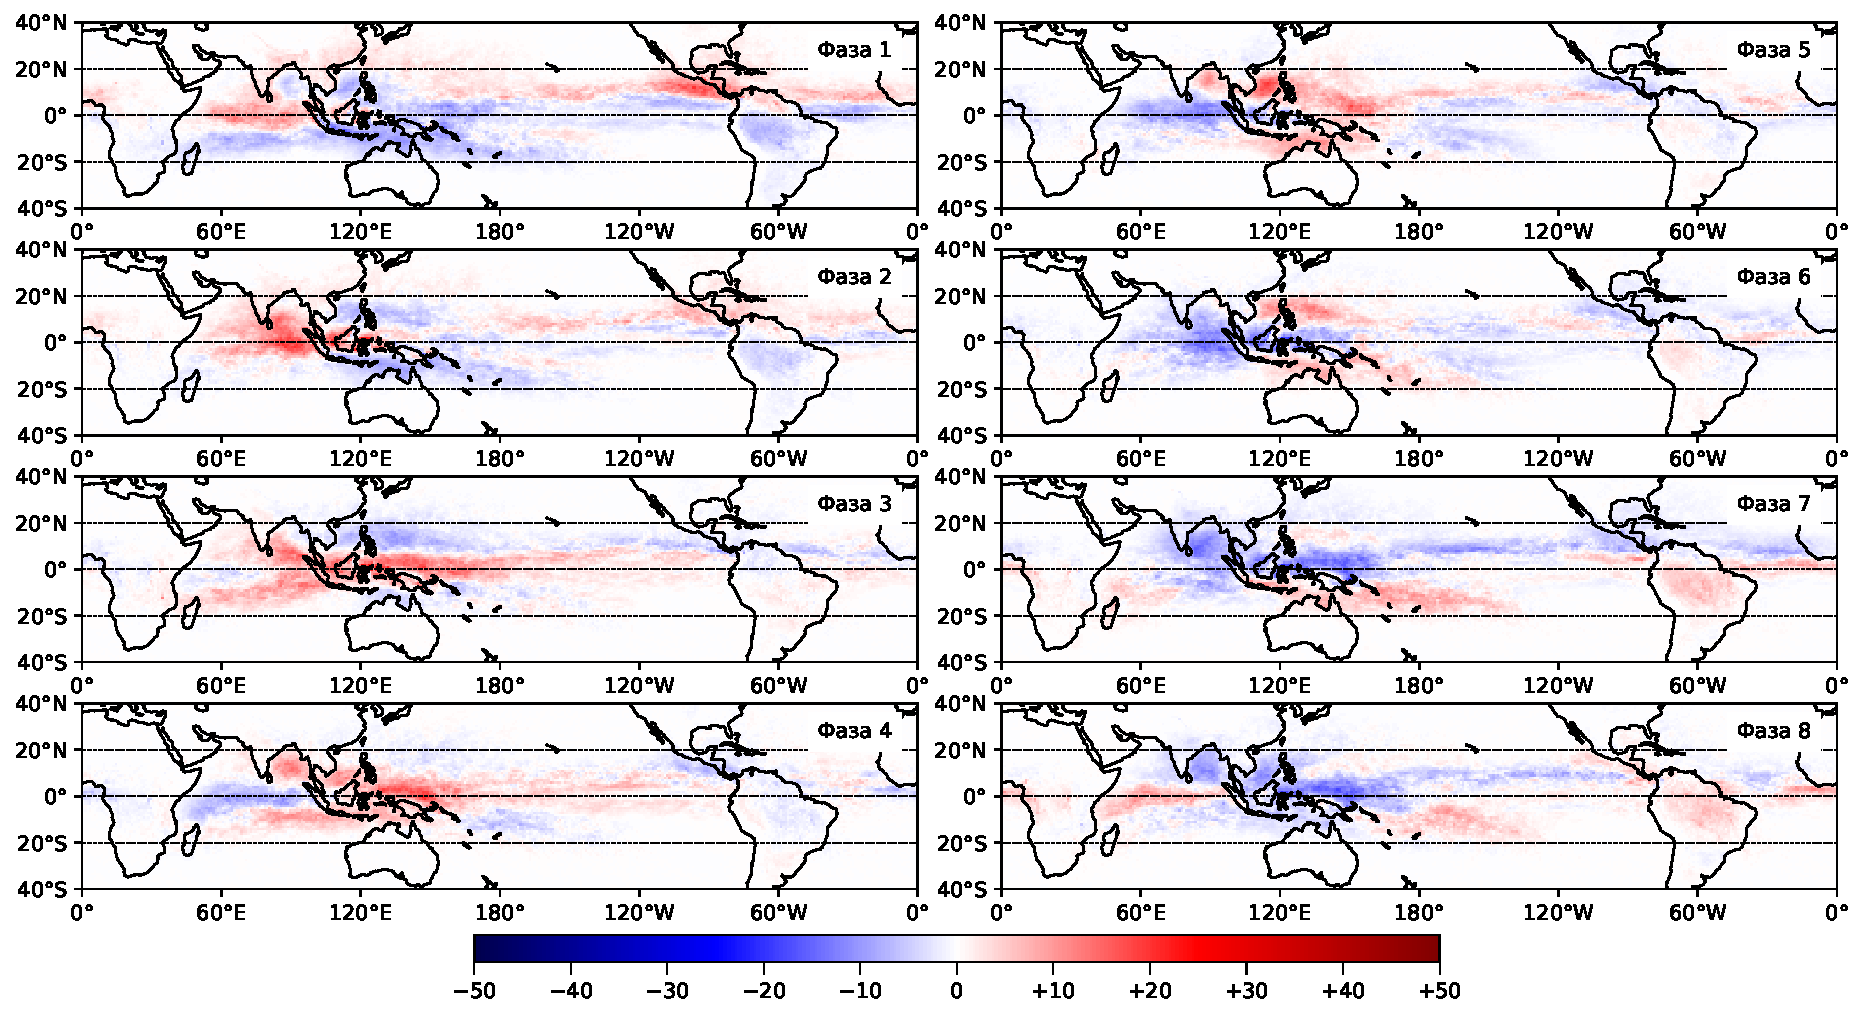
\includegraphics[width=\textwidth]{figures/map_of_contributions.pdf}
	\caption{Аномалии вкладов отдельных модельных столбцов в ИП (в вольтах) в течение каждой из фаз КМД.}
	\label{fig:map_of_contributions}
\end{figure}

Такие образом в среднем моделируемые вклады в ИП изменяются в соответствии с динамикой конвекции на масштабах КМД, что не должно быть удивительным ввиду используемой параметризации (\ref{eq:ip}). Гораздо более интересно было бы посмотреть на такой параметр модели ГЭЦ, как ИП. Рис. \ref{fig:variations}{a} показывает средние значения ИП в различные фазы КМД. Видно, что вариация имеет вид синусоиды с максимумом в 3 фазе и минимумом в 7 фазе. Период синусоиды близок к 8 фазам КМД, а амплитуда составляет $12\,\textnormal{кВ}$.

\begin{figure} 
    \centering
    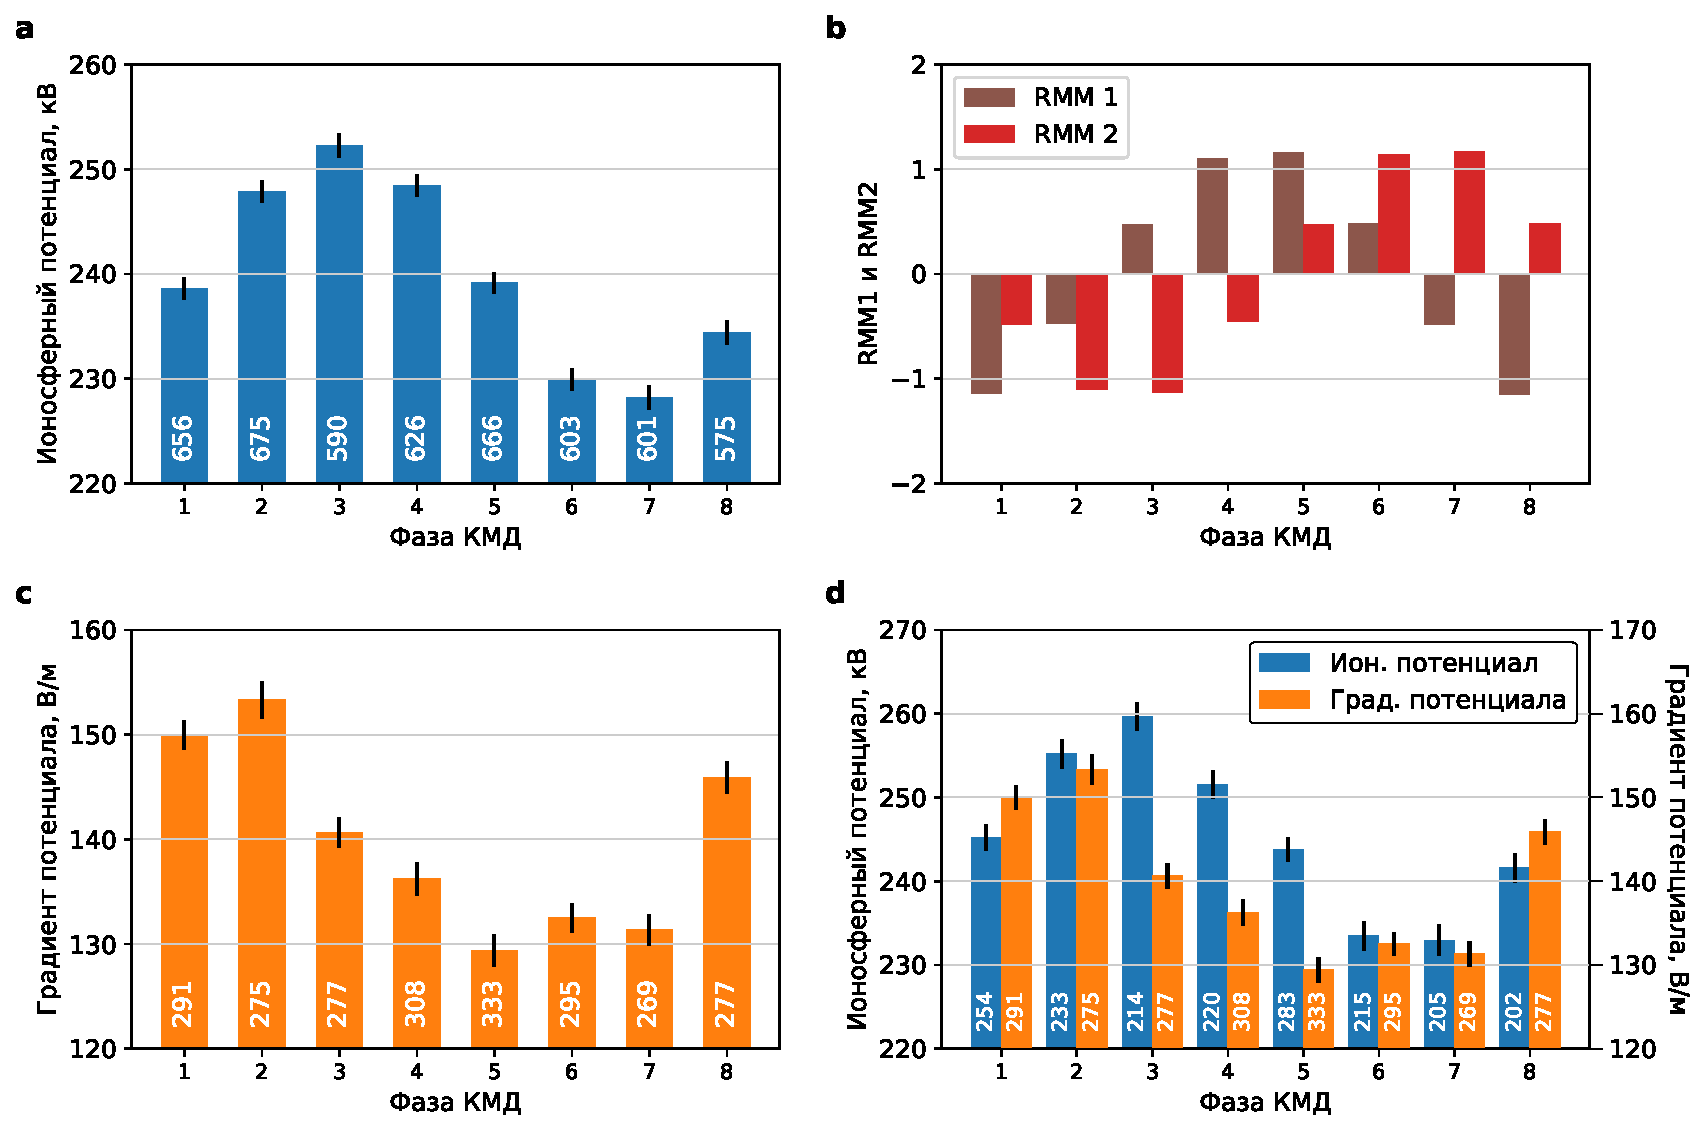
\includegraphics[width=\textwidth]{figures/variations.pdf}
    \caption{(a): Средние значения моделируемого ИП за каждую из фаз КМД (на основе моделирования за 1980--2020). (b): Средние значения компонент индекса RMM за каждую из фаз КМД на основе данных за 1980--2020. (c): Средние значения ГП, измеренного в хорошую погоду на станции Восток, для каждой из фаз КМД (на основе измерений в течение 2006--2020). (d): Сравнение значений ГП, показанных на панеле (c) со значениями моделируемого ИП за тот же временной интервал (2006--2020). Черные штрихи на столбцах на понелях (a), (c) и (d) обозначают плюс и минус одну стандартную ошибку, а числа в столбцах на тех же панелях указывают количество дней моделирования или измерений в хорошую погоду, которые пришлись на каждую из фаз КМД.}
    \label{fig:variations}
\end{figure}

Рис. \ref{fig:variations}{b} демонстрирует средние значения RMM1 и RMM2 в различные фазы КМД (на основе данных за 1980--2020). Такие вариации хорошо приближаются синусоидами, ведь фазы КМД возможно определять с помощью полярного угла на плоскости (RMM1, RMM2) (см. рис. \ref{fig:wh04_fig7}), который задаётся как $\arctg(\mathrm{RMM2}/\mathrm{RMM1})$. Вариации RMM1 и RMM2 имеют схожие амплитуды и сдвинуты друг относительно друга на четверть периода, что отражает тот факт, что усредненная по многим циклам КМД траектория состояния КМД на плоскости (RMM1, RMM2) близка к окружности.

Из сравнения рис. \ref{fig:variations}{b} и \ref{fig:variations}{a} можно заключить, что зависимость ИП от фазы КМД во многом повторяет зависимость RMM2 от фазы КМД, взятую с обратным знаком. Точнее, между этими вариациями есть сильная негативная корреляция с коэффициентом корреляции $r=-0.93$. В то же время коэффициент корреляции ИП с RMM1 составляет лишь $r=0.33$.

Рассматривается $N = 8$ фаз КМД. Можно оценить значимость наблюдаемой корреляции используя двухвыборочный t-критерий для независимых выборок Стьюдента с $N - 2 = 6$ степенями свободы. Если даны две независимые выборки размера $N$, а $r$~---~коэффициент корреляции между ними, то величина
\begin{equation}
 	q = \dfrac{r\sqrt{N-2}}{\sqrt{1-r^2}}
\end{equation}
точно подчиняется распределению Стьюдента. На уровне значимости 1\% гипотеза о том, что две выборки независимы отвергается, если $q\ge3.71$ или $\abs{r}\ge0.83$. Из данного критерия следует, что негативная корреляция между ИП и RMM2 ($r=-0.93$) статистически значима на уровне значимости 1\%, однако связь между ИП и RMM1 ($r=0.33$) не значима.

Если рассматривать данный вопрос более широко, то можно учесть двумерность индекса RMM, что позволяет вместо RMM1 и RMM2 рассматривать проекцию индекса RMM на любое направление в плоскости (RMM1, RMM2), то есть можно оперировать с величиной 
\begin{equation}\label{rmm_direction}
	\mathrm{RMM1}\cdot \cos\phi + \mathrm{RMM2}\cdot \sin\phi,
\end{equation}
где $\phi$~---~полярный угол на плоскости (RMM1, RMM2) (отсчитывается от положительного направления RMM1). Коэффициент корреляции между величиной (\ref{rmm_direction}) и ИП зависит от полярного угла $\phi$ так, как показано на рис. \ref{fig:r} (голубая кривая), и достигает своего максимального значения ($r=0.99$) при $\phi=290^\circ$; на рис. \ref{fig:rmm_diagram} это направление обозначено голубой пунктирной линией. Таким образом можно утверждать, что значения ИП, будучи усреднены по фазам КМД, крайне хорошо коррелируют с циклом КМД.

\begin{figure}[htbp]
	\centering
	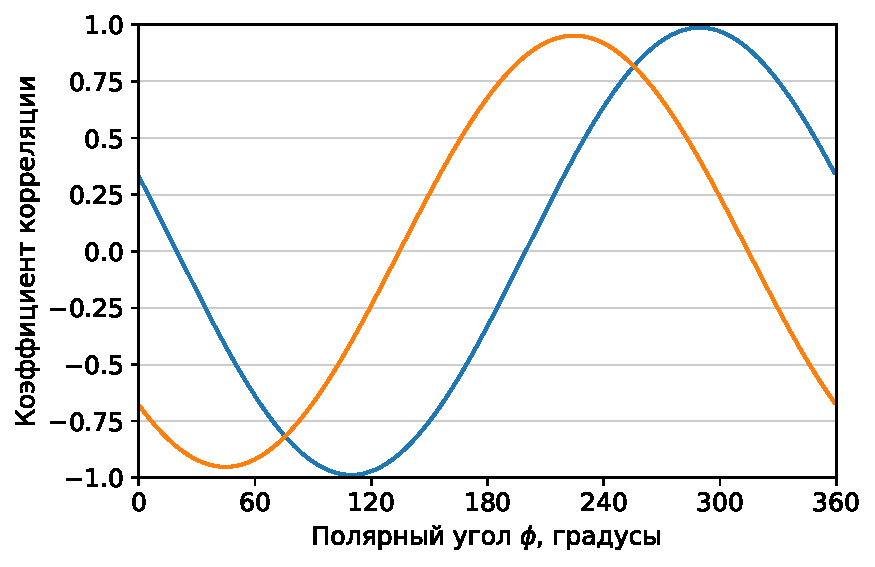
\includegraphics[width=0.6\textwidth]{figures/r.pdf}
	\caption{Коэффициент корреляции между величиной (\ref{rmm_direction}) и ИП (голубая линия), а также между величиной (\ref{rmm_direction}) и ГП (оранжевая линия) в зависимости от полярного угла $\phi$.}
	\label{fig:r}
\end{figure}

Стоит заметить, что направление в сторону отрицательных значений RMM2 соответствует полярному углу $\phi=270^\circ$, что близко к $\phi=290^\circ$, а направление в сторону положительных значений RMM1 соответствует $\phi=0^\circ$, что почти перпендикулярно к направлению $\phi=290^\circ$. Это согласуется с ранними результатами, согласно которым ИП негативно коррелирует с RMM2, но не коррелирует с RMM1.
